%% Author_tex.tex
%% V1.0
%% 2012/13/12
%% developed by Techset
%%
%% This file describes the coding for rsproca.cls

\documentclass[]{rsos}%%%%where rsos is the template name

\usepackage{lineno}
\linenumbers

\usepackage[T1]{fontenc}
\usepackage[utf8]{inputenc}


%%%% *** Do not adjust lengths that control margins, column widths, etc. ***

%%%%%%%%%%% Defining Enunciations  %%%%%%%%%%%
\newtheorem{theorem}{\bf Theorem}[section]
\newtheorem{condition}{\bf Condition}[section]
\newtheorem{corollary}{\bf Corollary}[section]
%%%%%%%%%%%%%%%%%%%%%%%%%%%%%%%%%%%%%%%%%%%%%%%

\begin{document}

%%%% Article title to be placed here
\title{Evolutionary simulations of \emph{Z}-linked suppression gene drives}

\author{
Luke Holman$^{1}$}

\address{
  $^{1}$School of BioSciences, The University of Melbourne, Victoria 3010,
Australia.}
%%%% Subject entries to be placed here %%%%
\subject{
Evolutionary biology,
Theoretical modelling,
Gene drives}

%%%% Keyword entries to be placed here %%%%
\keywords{
Sex chromosomes,
Gene drives,
Population control,
Schistosomiasis,
Selfish genes}

%%%% Insert corresponding author and its email address}
\corres{
  L. Holman\\
  e-mail: \href{mailto:luke.holman@unimelb.edu.au}{\nolinkurl{luke.holman@unimelb.edu.au}}
}

%%%% Abstract text to be placed here %%%%%%%%%%%%
\begin{abstract}
Synthetic gene drives may soon be used to suppress or eliminate
populations of disease vectors, pathogens, invasive species, and
agricultural pests. Recent proposals have focused on using
\emph{Z}-linked gene drives to control species with \emph{ZW} sex
determination, which include Lepidopteran pests, parasitic trematodes,
and cane toads. These proposals include \emph{Z}-linked
`\emph{W}-shredders', which would suppress populations by cleaving the
\emph{W} chromosome and causing females to produce only sons, as well as
\emph{Z}-linked female-sterilising gene drives. Here I use
eco-evolutionary simulations to evaluate the potential of some proposed
\emph{Z}-linked gene drives, and to produce recommendations regarding
their design and use. The simulations show that \emph{W}-shredders are
likely to be highly effective at eradicating populations provided that
resistance to \emph{W}-shredding cannot evolve. However,
\emph{W}-shredder alleles can invade populations from very low
frequencies, making it difficult to eliminate specific populations while
leaving nearby populations untouched; this issue may restrict their
possible uses.
\end{abstract}
%%%%%%%%%%%%%%%%%%%%%%%%%%%

%% Some pieces required from the pandoc template
\providecommand{\tightlist}{%
  \setlength{\itemsep}{0pt}\setlength{\parskip}{0pt}}
\providecommand{\EndFirstPage}{%
}

\maketitle

\hypertarget{introduction}{%
\section{Introduction}\label{introduction}}

Developments in genetic engineering will soon make it feasible to alter
or eliminate populations of disease vectors, pathogens, agricultural
pests, and invasive species using `gene drives'
\citep{gantz2015hi, hammond2016cr, wang2016cr, prowse2017do, kyrou2018cr, noble2018cu}.
Gene drives cause particular alleles (usually transgenes) to propagate
through populations via a range of mechanisms, including gene
conversion, poison-antidote systems, segregation distortion, and genetic
incompatibility \citep{lindholm2016ec, champer2016ch, oberhofer2019cl}.
For example, CRISPR-Cas9 gene editing can be used to create a transgene
that will be transmitted to almost 100\% of the offspring of
heterozygous individuals instead of the usual 50\%; this type of gene
drive functions by inducing a double-stranded DNA break at the
homologous wild type locus, which is then repaired using the transgene
as a template. Gene drives are often categorised into two types:
replacement drives, which aim to spread a human-beneficial allele
throughout a population (e.g.~a mosquito allele that interferes with the
tranmission of malaria \citep{gantz2015hi, marshall2015gene}), and
suppression drives, which reduce the size of a population (potentially
to extinction). Suppression drives typically work by using non-Mendelian
inheritance to spread alleles that cause lethality or sterility
\citep{hammond2016cr, kyrou2018cr, maselko2018ge}, or skew the offspring
sex ratio -- typically towards males
\citep{windbichler2008ta, galizi2014sy, beaghton2017ve, burt2018se, papathanos2018re}.

Recent theoretical papers have investigated the feasibility, efficacy,
and potential negative consequencies of various types of gene drives.
For example, Noble et al. \citep{noble2018cu} showed that the basic
version of a CRISPR-Cas9 gene drive might be highly invasive and could
rapidly spread to fixation across whole species, which is often an
undesirable outcome. Conversely, other models have concluded that gene
drives are likely to fail if populations can evolve resistance to their
effects \citep{drury2017cr, unckless2017ev}. The issue of resistance is
compounded because the standard implementation of CRISPR-Cas9 gene drive
(but perhaps not updated versions;
\citep{esvelt2014em, unckless2017ev, prowse2017do, kyrou2018cr}) tends
to create its own resistance alleles, e.g.~when the double-stranded
break induced by Cas9 is repaired using an alternative DNA repair
pathway (non-homologous end joining; NHEJ) instead of homology-directed
repair
\citep{gantz2015mu, gantz2015hi, hammond2016cr, wang2016cr, unckless2017ev}.
Given the potential safety, ethical, and sociopolitical concerns
surrounding gene drives, some models have focused on gene drives that
would go extinct after a time
\citep{min2017da, burt2018se, noble2019da}, would stay confined to
particular populations \citep{maselko2018ge, noble2019da}, and/or could
be reversed once they have spread \citep{vella2017ev}.

This paper focuses on the evolutionary dynamics of \emph{Z}-linked
suppression gene drives. The simulation is inspired by proposals for
various types of \emph{Z}-linked gene drives by Kevin Esvelt and
colleagues, as well as ongoing efforts to develop these \emph{Z} drives
(see \href{}{www.sculptingevolution.org}; at the time of writing, these
ideas have not been published elsewhere). Various \emph{Z}-linked
suppression drives proposed by Esvelt and colleagues are shown
schematically in Figure 1. Depending on its design, mode of action and
the biology of the target species, \emph{Z} chromosomes carrying the
drive allele (denoted \emph{Z*}) might enjoy a transmission advantage in
\emph{Z*W} females (Figure 1B, and perhaps also 1C), and optionally also
in \emph{Z*Z} males. Esvelt et al.~focus on using \emph{Z} drives to
control the \emph{Schistosoma} trematodes responsible for
schistosomiasis, though \emph{Z} drives could theoretically be used to
control any organism with female-heterogametic sex determination, such
as Lepidopteran agricultural pests, invasive populations of cane toads
\emph{Bufo marinus} \citep{abramyan2009z}, or even invasive birds.

A \emph{Z}-linked gene drive could suppress populations by biasing
gametogenesis in females, for example by inducing double-stranded DNA
breaks in the \emph{W} chromosome in order to inactivate it; such a gene
drive would be a `\emph{W}-shredder', analagous to the \emph{X}- and
\emph{Y}-shredders under development for \emph{XY} species
\citep{windbichler2008ta, north2013mo, galizi2014sy, burt2018se, papathanos2018re, prowse2019}.
Females carrying the gene drive would thus produce relatively few viable
\emph{W}-bearing eggs, and therefore produce mainly drive-carrying sons.
Esvelt et al.~point out that the evolutionary dynamics of the drive will
depend on the fitness of drive carriers relative to wild types, the
timing of \emph{W}-shredding (e.g.~in germ cells, ova, or zygotes), and
the ecology of the target species. For example, some \emph{W}-shredder
designs might allow drive females to produce roughly the same number of
(mostly-male) offspring as a wild-type female provided that the \emph{W}
chromosome is destroyed early enough in oogenesis/development that the
lost daughters can be replaced by sons (Figure 1B). Alternatively,
drive-carrying females might produce half the number of offspring (or
fewer), e.g.~if the drive works by destroying all ova or offspring that
carry a \emph{W} chromosome, and this loss is not compensated by reduced
competition on the surviving offspring. Esvelt et al.~also proposed that
one could suppress populations using a \emph{Z}-linked locus that caused
sterility or lethality in females, either by shredding the \emph{W} in
somatic tissues, or by spreading some other allele that harms females
but not males. If this female-harming allele were capable of gene drive
in males, it could perhaps reach high enough frequencies to suppress the
population. The \emph{W}-shredder could be designed to also cause gene
drive in males. Male gene drive could be accomplished using `standard'
CRISPR-Cas9 gene conversion, whereby the driving \emph{Z} allele would
convert the wild type locus using homing endonuclease activity followed
by homology-directed repair, causing heterozygous males to produce
mostly drive-carrying sperm. Esvelt et al.~note that male gene drive
might not be necessary, since a \emph{Z}-linked locus that prevents
transmission of the \emph{W} may already enjoy a transmission advantage
(Figures 1B-1C).

Here, I present an evolutionary simulation that can accommodate all of
these proposed \emph{Z}-linked drives. I aimed to test which properties
of the gene drive and the ecology of the target species are critical to
determining the likelihood and speed of extinction. For example, the
gene drive will presumably spread faster if it can bias transmission in
both sexes, but perhaps a simpler female-only drive would be adequate.
Also, since the population will become more male-biased as the gene
drive invades, eco-evo feedback might affect the outcome of the drive
release in non-intuitive ways. For example, alleles that prevent
\emph{W}-shredding might have an especially large fitness advantage
relative to resistance alleles against `standard' CRISPR drives
\citep[see][]{unckless2017ev, drury2017cr}, since the former restore a
normal sex ratio as well as defusing the harmful effect of the driver on
individual fitness. Moreover, the change in sex ratio could affect the
ecology and evolution of the population, particularly if males and
females contribute differentially to density-dependent population growth
\citep{rankin2007ma, li2019int}, or have different dispersal rates
\citep{li2019sex}. The model incorporates the possibility that
\emph{Z}-linked resistant-to-drive alleles are sometimes created by NHEJ
in heterozygote males, to test whether resistance is just as problematic
as for autosomal drives
\citep{gantz2015mu, gantz2015hi, hammond2016cr, wang2016cr, unckless2017ev}.

\hypertarget{methods}{%
\section{Methods}\label{methods}}

A full description of the simulation is provided as Supplementary
Material. In brief, I simulate a finite population of dioecious diploids
with \emph{ZW} sex determination that inhabits \(k\) discrete habitat
patches arranged linearly in a ring. The aim of the simulation is to
identify properties of the gene drive and the ecology of the target
species that influence the outcome of a single release of
\(n_{release}\) homozygote males carrying a \emph{Z}-linked gene drive
allele, \emph{Z*}. The drive allele causes biased inheritance and/or
reduced fecundity in females, and optionally also causes biased
inheritance in heterozygous males (e.g.~via gene conversion). Each
generation proceeds in discrete steps: birth, dispersal between patches,
breeding within patches, and death of the parental generation. The
equilibrium population size was roughly 10,000 in all simulations upon
release of the gene drive, and the main outcomes of interest are the
likelihood and speed of extinction. The simulation was written in R
3.4.0 and run on the Spartan cluster at the University of Melbourne;
Table 1 lists the simulation parameters that were manipulated to study
their effects.

Each male carries two diploid autosomal loci (termed \emph{A/a} and
\emph{B/b}) and one diploid \emph{Z}-linked locus, while females carry
both autosomal loci, a single allele at the \emph{Z}-linked locus, plus
a \emph{W} chromosome. There are three possible \emph{Z}-linked alleles:
the drive allele (\emph{Z*}), a wild-type allele (\(Z^+\)) that is
vulnerable to gene drive in \emph{Z*}\(Z^+\) males, and a resistant
allele (\(Z^r\)) that is immune to gene drive in \emph{Z*}\(Z^r\) males.
Similarly, there are two types of \emph{W} chromosome: a wild-type
\emph{W} that is vulnerable to shredding by the \emph{Z*} allele
(\(W^+\)), and an immune variant (\(W^r\)). The autosomal alleles
\emph{A} and \emph{B} are dominant `\emph{trans}-acting' resistance
alleles that confer immunity to \emph{W}-shredding and gene conversion,
respectively. The \emph{Z*} allele imposes a cost \(c_f\) on the
fecundity of female carriers, and a cost \(c_m\) on the mating success
of male carriers. The resistance alleles \(W^r\), \(Z^r\), \emph{A} and
\emph{B} are assumed to be cost-free. Setting \(c_f = 1\) allows
simulation of a female-sterilising \emph{Z}-linked drive (Figure 1D).

Females carrying \emph{Z*} (and no \emph{A} or \(W^r\) alleles) produce
\(\frac{1}{2}(1 + p_{shred})\) \emph{Z}-bearing gametes and
\(\frac{1}{2}(1 - p_{shred})\) \emph{W}-bearing gametes, and thus
produce \textgreater{}50\% sons when \(p_{shred} > 0\). Secondly,
\emph{Z*}\(Z^+\) males produce
\(\frac{1}{2}(1 + p_{conv} - p_{conv} p_{nhej})\) gametes carrying the
\emph{Z*} allele, \(\frac{1}{2}(1 - p_{conv})\) gametes carrying the
\(Z^+\) allele, and \(\frac{1}{2}(p_{conv} p_{nhej}))\) gametes carrying
the \(Z^r\) allele. Thus, gene conversion occurs in males if
\(p_{conv} > 0\), meaning that the \emph{Z*} allele is over-represented
in the gametes of these three male genotypes. The parameter \(p_{nhej}\)
represents the creation of resistance alleles via non-homologous end
joining.

Female fecundity depends on the local and/or global density and fitness
of other females, and the density of males, via functions involving five
parameters that control the carrying capacity (\(K\)), maximum possible
fecundity (\(r\)), the shape of the density-dependence function
(\(\alpha\)), the relative effect of males and females on density
(\(\delta\)), and the scale of density-dependence (local or global;
\(\psi\)). These parameters allow the model to capture a range of
possible life histories suitable for different organisms that could be
suppressed with \emph{W}-shredders. For example, maximum fecundity \(r\)
is lower for birds than for cane toads, and \(\delta\) might be lower in
Lepidoptera than trematodes, since male trematodes consume
space/resources inside the host (and males are much larger than
females), while male Lepidoptera do not consume one of the main limitied
resources that females need (i.e.~host plants on which to lay their
eggs). Female and male offspring disperse to other patches with
probabilities \(x_f\) and \(x_m\) respectively, allowing for variable
and sex-specific gene flow between patches. Dispersal was either local
or global (i.e.~to a neighbouring patch or a random patch).

\hypertarget{results}{%
\section{Results}\label{results}}

\hypertarget{three-illustrative-simulation-runs}{%
\subsection{Three illustrative simulation
runs}\label{three-illustrative-simulation-runs}}

Figure 2 shows three contrasting simulation runs. In Figure 2A, the
release of \emph{Z*Z*} males at generation 50 caused the \emph{Z*}
allele in invade and fix, causing rapid extinction due to a lack of
females. The simulation run in Figure 2A assumed that \emph{Z*} causes
near-complete \emph{W}-shredding, \emph{Z*} benefits from gene drive in
males, that \emph{Z*} has modest fitness costs to carriers, and there is
no resistance to \emph{W}-shredding (Table S1).

In Figure 2B, \emph{Z*} went to fixation but failed to cause extinction,
due to incomplete \emph{W}-shredding by the \emph{Z*} allele. In this
run, \(p_{shred} = 0.84\) (Table S1), meaning that 8\% of the offspring
of \emph{Z*}\(W^+\) mothers are female. The invasion of \emph{Z*}
altered the population sex ratio, but did not cause extinction (or even
a decline in population size).

Lastly, Figure 2C shows a case where the invasion of \emph{Z*} was
reversed by the evolution of autosomal resistance alleles. Following the
release of the \emph{Z*} allele, the initially rare autosomal resistance
allele \emph{A} (which prevents \emph{W}-shredding) rapidly increased in
frequency, disarming the effects of \emph{Z*} in females and returning
the population-level sex ratio to 50:50, even though the \emph{Z*}
allele reached fixation. Incidentally, the resistant allele \emph{A} was
favoured over \emph{a} because the male-biased population sex ratio
created by \emph{Z*} favours the production of daughters, and \emph{AA}
and \emph{Aa} females produce more daughters than \emph{aa} females in
populations where \emph{Z*} is present.

\hypertarget{effects-of-each-parameter-on-the-evolution-of-a-w-shredder}{%
\subsection{\texorpdfstring{Effects of each parameter on the evolution
of a
\emph{W}-shredder}{Effects of each parameter on the evolution of a W-shredder}}\label{effects-of-each-parameter-on-the-evolution-of-a-w-shredder}}

Figure 3 shows the effects of each parameter for simulations of a
\emph{Z}-linked \emph{W}-shredder allele that also potentially causes
gene drive in \emph{Z*Z} males. Figure 3 assumes complete
\emph{W}-shredding (\(p_{shred} = 1\)), because initial trials revealed
that extinction almsot never occurred if \(p_{shred} < 0.95\) (Figure
S1). This result confirms that a \emph{W}-shredder needs to effectively
prevent female carriers from producing daughters in order to reliably
cause extinction. Otherwise, all the parameters were allowed to vary
within pre-specified limits using Latin hypercube sampling. Thus, the
relationships in Figure 3 show the expected effect of the focal
parameter on extinction probability, while the other parameters vary
independently within the ranges shown on the \(x\)-axis of Figure 3.
Figure 4 is similar to Figure 3, except that it plots the average time
until extinction (for the subset of runs in which extinction actually
occurred).

\hypertarget{gene-drive-parameters}{%
\subsubsection{Gene drive parameters}\label{gene-drive-parameters}}

Extinction probability declined sharply as the costs of the gene drive
to female fecundity (\(c_f\)) and male mating success (\(c_m\))
increased, suggesting that one should work to minimise such costs when
developing a \emph{W}-shredder. Consistent with this conclusion, time
until extinction increased monotonically with the cost of male mating
success \(c_m\), but interestingly, the relationship between \(c_f\) and
the speed of extinction was hump-shaped. \emph{W}-shredders with no
costs in females caused extinction quickly due to their more rapid
spread, while \emph{W}-shredders that carried a sufficiently high cost
to females actually resulted in faster extinction (though note that
extinction rarely occurred when \(c_f\) was high), since female
fecundity is critical to population growth. On balance, the model
suggests that \emph{W}-shredders should be designed to have minimal
impact of the fitness of carriers, though reassuringly (from a design
standpoint), extinction still occurred frequently even if carriers were
10-20\% less fit than wild types.

Another very important parameter was the presence/absence of autosomal
resistance alleles that prevent \emph{W}-shredding from occurring:
extinction almost never happened when such alleles were present. Perhaps
surprisingly, when I allowed wild-type \(W^+\) chromosomes to mutate to
a resistant type, ensuring the population almost always contained a
small number of resistant \(W^r\) chromosomes, the probability of
extinction was essentially unaffected. The difference in outcome
relative to the \emph{A} allele may have to do with the reduced
population size of the \emph{W} chromosome, which is limited to females,
whose population size drops very rapidly once the \emph{Z*} allele
invades (Figure 2).

Extinction was substantially more likely when the \emph{W}-shredder was
also capable of gene drive in \emph{Z*Z} males. Although male gene drive
was non-essential for the \emph{W}-shredder to cause extinction,
efficient male-acting drive greatly reduced the number of generations
required for extinction to occur (see inset of Figure 4). Similarly,
resistance to the male-acting component of the gene drive reduced the
extinction probability (and increased the time until extinction),
especially when resistance alleles were created by non-homologous end
joining rather than arising randomly by mutation (presumably because the
latter causes the resistance alleles to appear in the same patches as
the drive allele, where they immediately enjoy a selective advantage).

The number of \emph{Z*Z*} males released into the population had little
effect on extinction probability: releasing 20 individuals was almost as
likely to cause extinction as releasing 100. This result reflects the
classic population genetics result that the fixation probability of a
strongly-selected allele (such as a gene drive) does not depend on its
frequency \citep[only on selection and population structure; reviewed
in][]{patwa2008fix}. Additionally, releasing the drive-carrying males
throughout the meta-population was equally likely to cause extinction as
releasing them all in one patch. As well as suggesting that multi-site
release programs might not be strictly necessary, this result implies
that \emph{Z}-linked gene drives are very likely to spread between
populations connected by gene flow, as previously found for autosomal
drives \citep{noble2018cu}.

\hypertarget{ecological-drive-parameters}{%
\subsubsection{Ecological drive
parameters}\label{ecological-drive-parameters}}

The most important ecological parameter was the number of patches into
which the population was divided. Spatially structured populations were
harder to drive extinct, presumably because the population can persist
in habitat patches where the drive allele is absent, and because
migrants can recolonise patches where local extinction has occurred.
Since patches containing the gene drive will produce fewer migrants (due
to their imbalanced sex ratio), migrants that recolonise empty patches
are more likely to carry wild-type or drive-resistant alleles. The time
until extinction increased with the patchiness of the population, with
diminishing returns.

Interestingly, the migration rate had a sex-specific relationship with
extinction probability. Extinction became increasingly likely as the
male migration rate (\(x_m\)) increased, since the drive allele is
primarily carried by males due to its effect on the sex ratio.
Conversely, the effect of the female migration rate (\(x_f\)) was
U-shaped. With very high female migration rates, population structure is
much reduced, ensuring that the drive allele quickly reaches any patch
that lacks it. With low female migration rates, the gene drive causes
local extinctions faster than patches can be recolonised by dispersal.
Intermediate rates of female dispersal allow for the creation of
long-lasting refugia from the drive allele, and also allow for some
recolonisation, resulting in a reduced probability of extinction.

Unsurprisingly, extinction was more likely when the maximum possible
fecundity of each female (\(r\)) was lower. However, the decline was not
linear, and the results suggest that \emph{W}-shredders are capable of
eliminating even those species in which a handful of surviving females
can rapidly repopulate. The results also suggest that extinction was
slightly more probable when female fecundity was determined primarily by
local rather than global density (\(\psi\)). This is because local
density can remain high (and thus, per-female fecundity can remain low)
even in meta-populations that are declining due to the spread of the
\emph{Z*} allele in some of their sub-populations.

The parameter \(\delta\), which represents sex differences in ecological
niche use and behaviour, had a hump-shaped relationship with extinction
probability. Low \(\delta\) indicates that female fecundity is only
weakly affected by the density of males, and this scenario was
associated with lower extinction probabilities. This is because the gene
drive creates male-biased populations, boosting female fecundity for any
given population size, and helping to stave off extinction. Conversely
when \(\delta\) is high, male density has a stronger negative effect on
female fecundity, which slightly reduced the probability of extinction
(perhaps because patches containing many drive alleles are male-biased,
and thus send out comparatively few drive-carrying migrants when
\(\delta\) is high). Extinction was most likely for intermediate values
of \(\delta\). By contrast, the time until extinction declined
monotonically with \(\delta\), since high values of \(\delta\) mean that
male-biased populations produce even fewer offspring.

Finally, the parameter \(\alpha\), which controls the shape of the
relationship between female fecundity and population density, had a weak
negative effect on the likelihood or speed of extinction. Setting
\(\alpha < 1\) means that female fecundity declines at a decelerating
rate as population density increases, such that per-female fecundity
only approaches its maximum possible value once the population is
heavily depleted, making extinction more likely.

\hypertarget{well-designed-w-shredders-cause-rapid-extinction}{%
\subsection{\texorpdfstring{Well-designed \emph{W}-shredders cause rapid
extinction}{Well-designed W-shredders cause rapid extinction}}\label{well-designed-w-shredders-cause-rapid-extinction}}

The inset of Figure 4 shows the frequency distribution for time until
extinction. With a well-designed \emph{W}-shredder and favourable
ecological conditions, the \emph{Z*} allele caused extinction in as few
as 9 generations. When considering only those simulations in which
\(p_{shred} = 1\) (i.e.~drive females produce no daughters) and the
fitness of drive carriers was within 5\% of the wild type, extinction
occurred within 20 generations for the majority of the parameter space
shown in Figures 3-4, illustrating that a well-designed
\emph{W}-shredder is likely to succeed in controlling species with very
different ecologies.

\hypertarget{female-sterilising-z-linked-gene-drive}{%
\subsection{\texorpdfstring{Female-sterilising \emph{Z}-linked gene
drive}{Female-sterilising Z-linked gene drive}}\label{female-sterilising-z-linked-gene-drive}}

For runs in which the \emph{Z*} allele caused females to become sterile
rather than biasing the offspring sex ratio (i.e. \(c_f = 1\)),
extinction never occurred (in 1,559,817 simulation runs). This was true
even when all other parameters besides \(c_f\) took values that make
extinction more likely, e.g.~when \emph{Z*} allele was transmitted to
100\% of the offspring of male heterozygotes, and when \emph{Z*} did not
harm male fitness. The reason for this result is that the fitness gains
from gene drive in males were not compensated by a complete loss of
fitness in females, at least for the ecological conditions considered
here. I hypothesise that a female-sterilising \emph{Z*} allele might be
capable of causing extinction if \emph{Z*} males were continuously
released into the population, but this possibility is outside the scope
of the model implemented here.

\hypertarget{discussion}{%
\section{Discussion}\label{discussion}}

The model shows that \emph{W}-shredders are, in principle, very
effective at eliminating populations, particularly if they fully prevent
females from producing daughters (\(p_{shred} \approx 1\)) and if
resistance to \emph{W}-shredding cannot evolve. The results have
implications for the design of \emph{Z}-linked \emph{W}-shredders and
female-sterilising suppression drives, and help to identify ecological
parameters that are (and are not) important to the outcome of a gene
drive release.

A major design consideration is whether to engineer \emph{W}-shredders
that are also capable of gene drive in males, e.g.~by including guide
RNAs that target the \emph{Z} as well as the \emph{W} chromosome, to
allow gene conversion in male heterozygotes. Foregoing male drive could
simplify the design of \emph{W}-shredders since they would only need to
target the \emph{W} chromosome (and not also the \emph{Z}), particularly
because male-acting gene conversion drives seem more challenging to
develop than female-acting ones in some taxa \citep[due to sex
differences in DNA repair;][]{grunwald2019super}). In the model,
\emph{W}-shredders very often caused extinction even without male gene
drive (i.e.~when \(p_{conv} \approx 0\)), provided that individuals
carrying the \emph{W}-shredder had comparable fitness to wild types, and
that carrier females produce very few daughters (as in Figure 1B).
Conversely if \emph{W}-shredder females had low fecundity (around half
that of a wild type, or below; Figure 1C) or produced some daughters,
male gene drive tended to be essential for extinction to occur, or at
least for extinction to occur rapidly enough to be useful. Although male
gene drive was not always needed for extinction to occur, it did
substantially reduce the number of generations until extinction.
Therefore, I conclude that it would almost certainly be worth the effort
to incorporate a male-acting component when developing a
\emph{W}-shredder, especially in species with longer generation times.

Another aim when designing \emph{W}-shredders should be to ensure that
female carriers produce as few daughters as possible (ideally none;
represented in the model as \(p_{shred}=1\)), while producing a large
number of drive-carrying sons (ideally as many as the total offspring
produced by non-carriers; \(c_f=0\)). This implies that one should aim
to design a construct that cleaves the \emph{W} chromosome early in
gametogenesis or offspring development, to increase the chance that the
number of surviving progeny produced by each female is unaffected.
Expression of Cas9 and cleavage of the \emph{W} should also be
restricted to the tissues where it is needed (e.g.~the germ line), to
minimise fitness losses due to the loss of the \emph{W} in somatic
cells, or detrimental effects of Cas9. For some species, this may be as
simple as placing the \emph{W}-shredder under the control of a promoter
such as \emph{nanos} \citep{champer2018re, zhang2018si}, assuming that
females are able to replace lost \emph{W}-bearing oocytes before they
are provisioned with limiting resources. Even if the lost daughters are
not replaced with additional sons, the \emph{Z*} allele might still
exhibit super-Mendelian inheritance across generations, because
\emph{Z*}-bearing males will experience reduced competition due to the
deaths of their sisters \citep[somewhat like the selfish genetic element
\emph{Medea};][]{hay2010en}). In Lepidoptera, juvenile density is often
strongly negatively correlated with survival, and there are various
maternally-transmitted endosymbionts that drive through populations by
killing males to lessen competition on their infected sisters (e.g.
\citep{jiggins2000bu, jiggins2003ma}); these observations suggest that
\emph{W}-shredder alleles might drive through Lepidopteran populations
even if \emph{Z*W} females produced half as many viable eggs, though
male gene drive would certainly help the invasion. The model also
highlighted that strong fitness costs to males (\(c_m\)) hinder the
spread of the drive allele, though it seems unliekly that a
\emph{W}-shredder allele would have major costs in males.

The \emph{W}-shredding mechanism should also be designed in a way that
makes it difficult for \emph{W}-linked or \emph{trans}-acting resistance
to shredding to evolve. One way to do this would be to use a single
guide RNA that targets \emph{W}-specific sequences that are present in
multiple copies, or to use multiple guide RNAs that target multiple
\emph{W}-linked sequences \citep{champer2018re, oberhofer2018be}; the
former is similar to the \emph{X}-shredder developed for
\emph{Anopheles} mosquitos, which cleaves repetitive, \emph{X}-linked
ribosomal genes \citep{galizi2014sy}. By designing gene drives with
multiple targets, the reference sequence must evolve multiple changes to
acquire resistance to cleavage, which is relatively unlikely. To ensure
that the targets of cleavage do not become resistant as a result of
indels induced by NHEJ, one can ensure that the guide RNA's target lies
within an essential gene where an indel would be selectively
disadvantageous, preventing resistant alleles from accumulating in the
population \citep{champer2018re, oberhofer2018be}. This may not be
necessary if the \emph{W}-shredder targets many \emph{W}-linked loci,
but it is an important design consideration for the male gene drive
component of the \emph{W}-shredder, because the evolution of
\emph{Z}-linked resistance completely nullified the usefulness of male
gene drive in the simulation (echoing \citep{unckless2017ev}). Recent
work demonstrated the feasibility of arrays containing many guide RNAs
separated by spacers \citep{kurata2018hi}, suggesting it may soon be
easier to create gene drives with multiple guide RNAs. A final way of
developing resistance is to `disarm' the endonuclease responsible for
\emph{W}-shredding and gene conversion, for example by producing a
protein that inhibits \emph{Cas9}, or through evolution of gene
regulatory processes that cause the \emph{Cas9} to no longer be
expressed at the right time. There appears to be little data on whether
this type of resistance is possible or likely, though models such as the
present one indicate that they could certainly impede population
suppression efforts.

The model also indicated that extinction does not require the release of
large numbers of individuals: releasing just 20 \emph{Z*} males was
often enough to eliminate a spatially-structured metapopulation of
10,000 individuals in a few generations. On the one hand, this is
advantageous because \emph{W}-shredders would be cheap and easy to
deploy once they are developed, and they are likely to extirpate whole
metapopulation even if gene flow between sites is quite weak. However,
such high invasiveness is not always desirable, because it makes the
gene drive very difficult to restrict to a particular area. This could
limit the usefulness of \emph{W}-shredders to control species like
Lepidoptera and birds, where one may wish to eradicate only invasive or
agriculturally damaging populations, while leaving other populations
untouched. Modifications to gene drive design -- such as the
self-limiting `daisy drive' system -- might someday address this
important concern \citep{min2017da, noble2019da}.

The model found several ecological variables that affect the likelihood
of extinction, but reassuringly the effects on extinction probability
were somewhat minor, and I found no ecological parameter values that
made extinction impossible. Populations in which females can produce
many offspring (high \(r\)) were harder to drive extinct, though the
effect of \(r\) reached an asymptote around \(r = 250\), such that even
extremely fecund organisms could be controlled using \emph{W}-shredders:
this is because fecundity doesn't matter if the population is all-male.
Patchy populations were harder to drive extinct, though this could
probably be mitigated by releasing gene drive individuals in larger
numbers, over a greater range, over multiple releases. Dispersal was a
double-edged sword: weak gene flow meant that the gene drive spread more
slowly through the meta-population, while high dispersal rates allow for
re-colonisation of patches in which the gene drive had caused
extinction. Demographic parameters such as the scale of competition
(\(\psi\)) and the shape of density-dependence (\(\alpha\)) mattered
little. Perhaps surprisingly, the relative importance of male density to
population growth (\(\delta\)) had only a weak effect: extinction was a
little more likely when the presence of males suppresses female
fecundity just as much (or more so) as the presence of other females.
However, extinction still occurred when female fecundity depended only
weakly on male density (again, probably because female fecundity becomes
unimportant as females begin to disappear from the population).

Finally, I note that \emph{W}-shredders might in general be easier to
develop than \emph{X}-shredders. Efforts to develop an \emph{X}-shredder
in \emph{Anopheles} mosquitos were initially hindered because the I-PpoI
protein used to cleave the \emph{X} was paternally transmitted to the
embryo inside sperm, causing all of the drive male's offspring to die
(not just the daughters) due to cleavage of the maternally-inherited
\emph{X} in the male's sons. Although this technical issue was later
addressed \citep{galizi2014sy}, such intergenerational effects would not
hinder a \emph{W}-shredder since the \emph{W} chromosome is unique to
females (provided that the \emph{W}-shredding protein was not expressed
in males, or at least was absent from their sperm). Additionally,
\emph{W}-shredders might sometimes be easier to develop than gene drives
that work by deleting genes that are essential to female (but not male)
fitness \citep[e.g.][]{burt2018se}. This is because one could design a
prototype \emph{W}-shredder based only on sequence data from the sex
chromosomes, while identifying genes with female-specific fitness
effects requires more detailed data (e.g.~expression profiling or
knockout studies) that are unavailable for most taxa.

\newpage

\hypertarget{tables}{%
\section{Tables}\label{tables}}

\textbf{Table 1}: List of variables, and their corresponding
parameter(s) in the model, which were varied in order to study their
effects on extinction.

\begin{table}[ht]
\centering
\begin{tabular}{ll}
  \hline
Variable & Parameter(s) \\ 
  \hline
Strength of gene drive in females (e.g. \textit{W}-shredding) & $p_{shred}$ \\ 
  Strength of gene drive in males (e.g. gene conversion) & $p_{conv}$ \\ 
  Cost of gene drive allele to female fecundity & $c_f$ \\ 
  Cost of gene drive allele to male mating success & $c_m$ \\ 
  Frequency of \textit{W}-linked resistance mutations & $\mu_W$ \\ 
  Frequency of \textit{Z}-linked resistance mutations and NHEJ & $\mu_Z$ and $p_{nhej}$ \\ 
  Frequency of autosomal resistance alleles & $\mu_A$ and $\mu_B$ \\ 
  Patchiness of the population & $k$ \\ 
  Dispersal rate of males and females & $x_m$ and $x_f$ \\ 
  Global versus local density-dependence of female fecundity & $\psi$ \\ 
  Contribution of males relative to females in density-dependence & $\delta$ \\ 
  Number of gene drive carrier males released & $n_{release}$ \\ 
  Release strategy: all in one patch, or global & - \\ 
  Fecundity of females at low population densities & $r$ \\ 
  Shape of density dependence & $\alpha$ \\ 
   \hline
\end{tabular}
\end{table}

\newpage

\hypertarget{figures}{%
\section{Figures}\label{figures}}

\begin{figure}[h]
\centering
\includegraphics[width=1.0\textwidth]{../figures/figure1_moths.pdf}
\caption{\footnotesize{Some hypothetical \textit{Z}-linked suppression drives considered in this study. Panel A illustrates normal inheritance of sex chromosomes in a wild type \textit{ZW} female (assumed to be mated to a wild type \textit{ZZ} male; not shown): the offspring sex ratio is even. In panel B, the female carries a \textit{W}-shredder allele ($Z^*$) that kills gametes or offspring early enough that missing daughters are replaced with more $Z^*$-bearing sons. In panel C, the lost daughters are not replaced, though their absence increases the survival probability of the sons somewhat (shown by their larger size), causing super-Mendelian inheritance of the $Z^*$ allele. Lastly, panel D shows a \textit{Z}-linked female-sterilising allele (e.g. an allele that cleaves the \textit{W} chromosome or a female-essential gene in somatic cells); since it is strongly disadvantageous in females, such an allele would go extinct unless it benefits from gene drive in heterozygous males.}}
\end{figure}
\newpage

\begin{figure}[h]
\centering
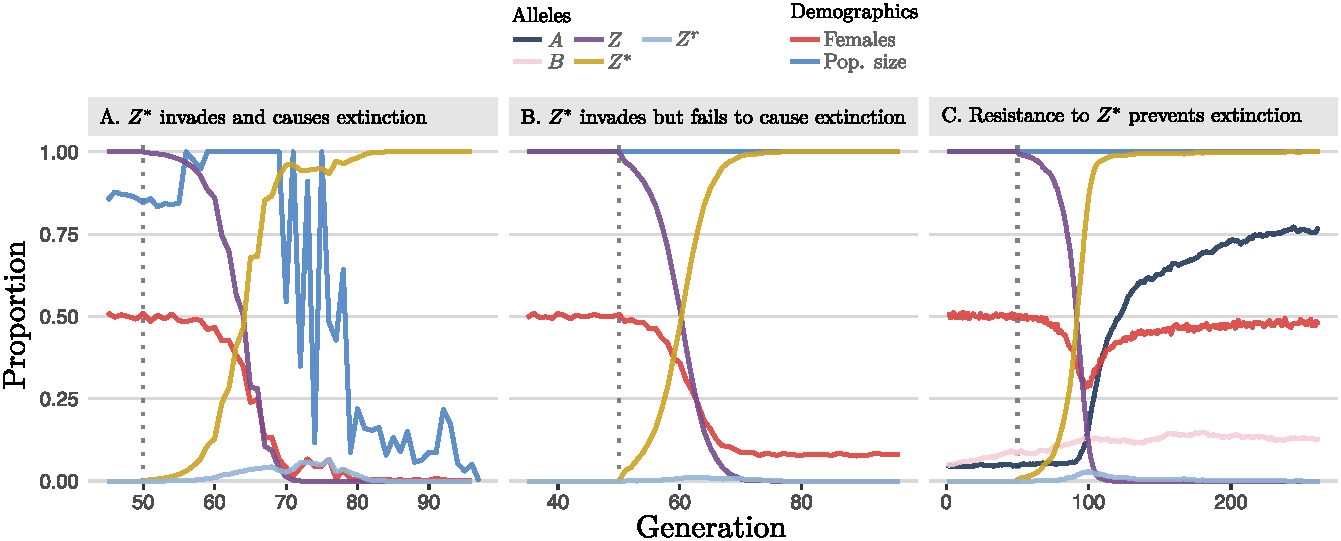
\includegraphics[width=1.0\textwidth]{../figures/fig_2_inkscape.pdf}
\caption{\footnotesize{Three illustrative runs of the simulation, showing evolution in response to the release of males carrying a \textit{W}-shredder at Generation 50 (dotted line). In panel A, the driving $Z^*$ allele fixed very quickly, causing population extinction through a shortage of females. In panel B, the $Z^*$ allele fixed but did not cause extinction, because carrier females continued to produce some daughters due to incomplete \textit{W}-shredding. In panel C, the $Z^*$ allele invaded, which selected for the \textit{W}-shredding resistance allele \textit{A}, causing $Z^*$ to go extinct by removing its transmission advantage. The population size \textit{N} is shown as a fraction of its maximum value of 10,000. Table S1 lists the parameter spaces used for these three runs.}}
\end{figure}
\newpage

\begin{figure}[h]
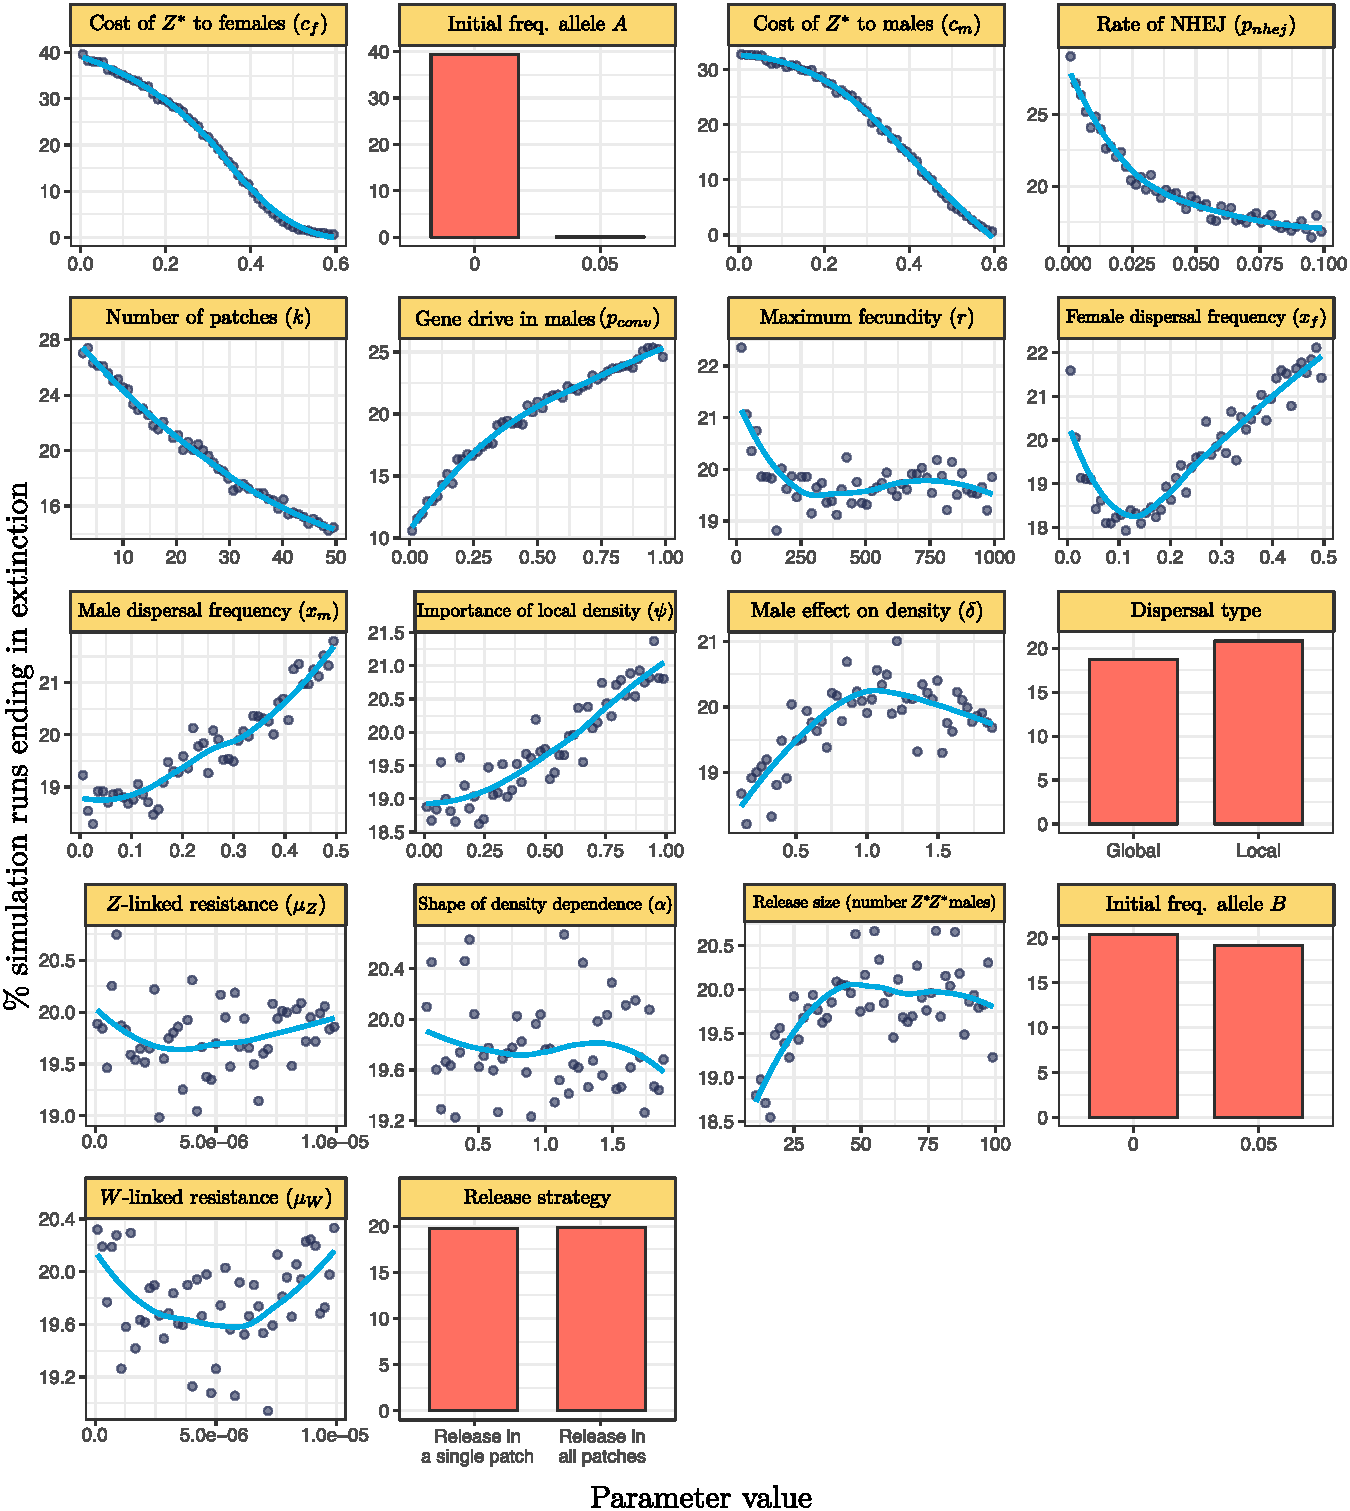
\includegraphics[width=1.0\textwidth]{../figures/fig_3_inkscape.pdf}
\caption{\footnotesize{The plot shows the effect of each model parameter on the percentage of simulation runs in which the population went extinct, for simulations of a \textit{Z}-linked \textit{W}-shredder that completely prevents the production of daughters by females ($p_{shred} = 1$; see also Figure S1). The plot was generated by sampling evenly from the complete parameter space 721,587 times using Latin hypercube sampling, such that each plot shows the marginal effect of one parameter while the other parameters vary independently across their possible ranges (shown by the relevant $x$-axis scale). Continuous parameters were grouped into 51 bins (each containing \textit{c.} 14,400 runs, 2\% of the total), and the lines were fitted using LOESS (locally estimated scatterplot smoothing). Note that the $y$-axis scales to the range of the data, and the panels are ordered by this range (showing the approximate relative importance of each parameter).}}
\end{figure}
\newpage

\begin{figure}[h]
\centering
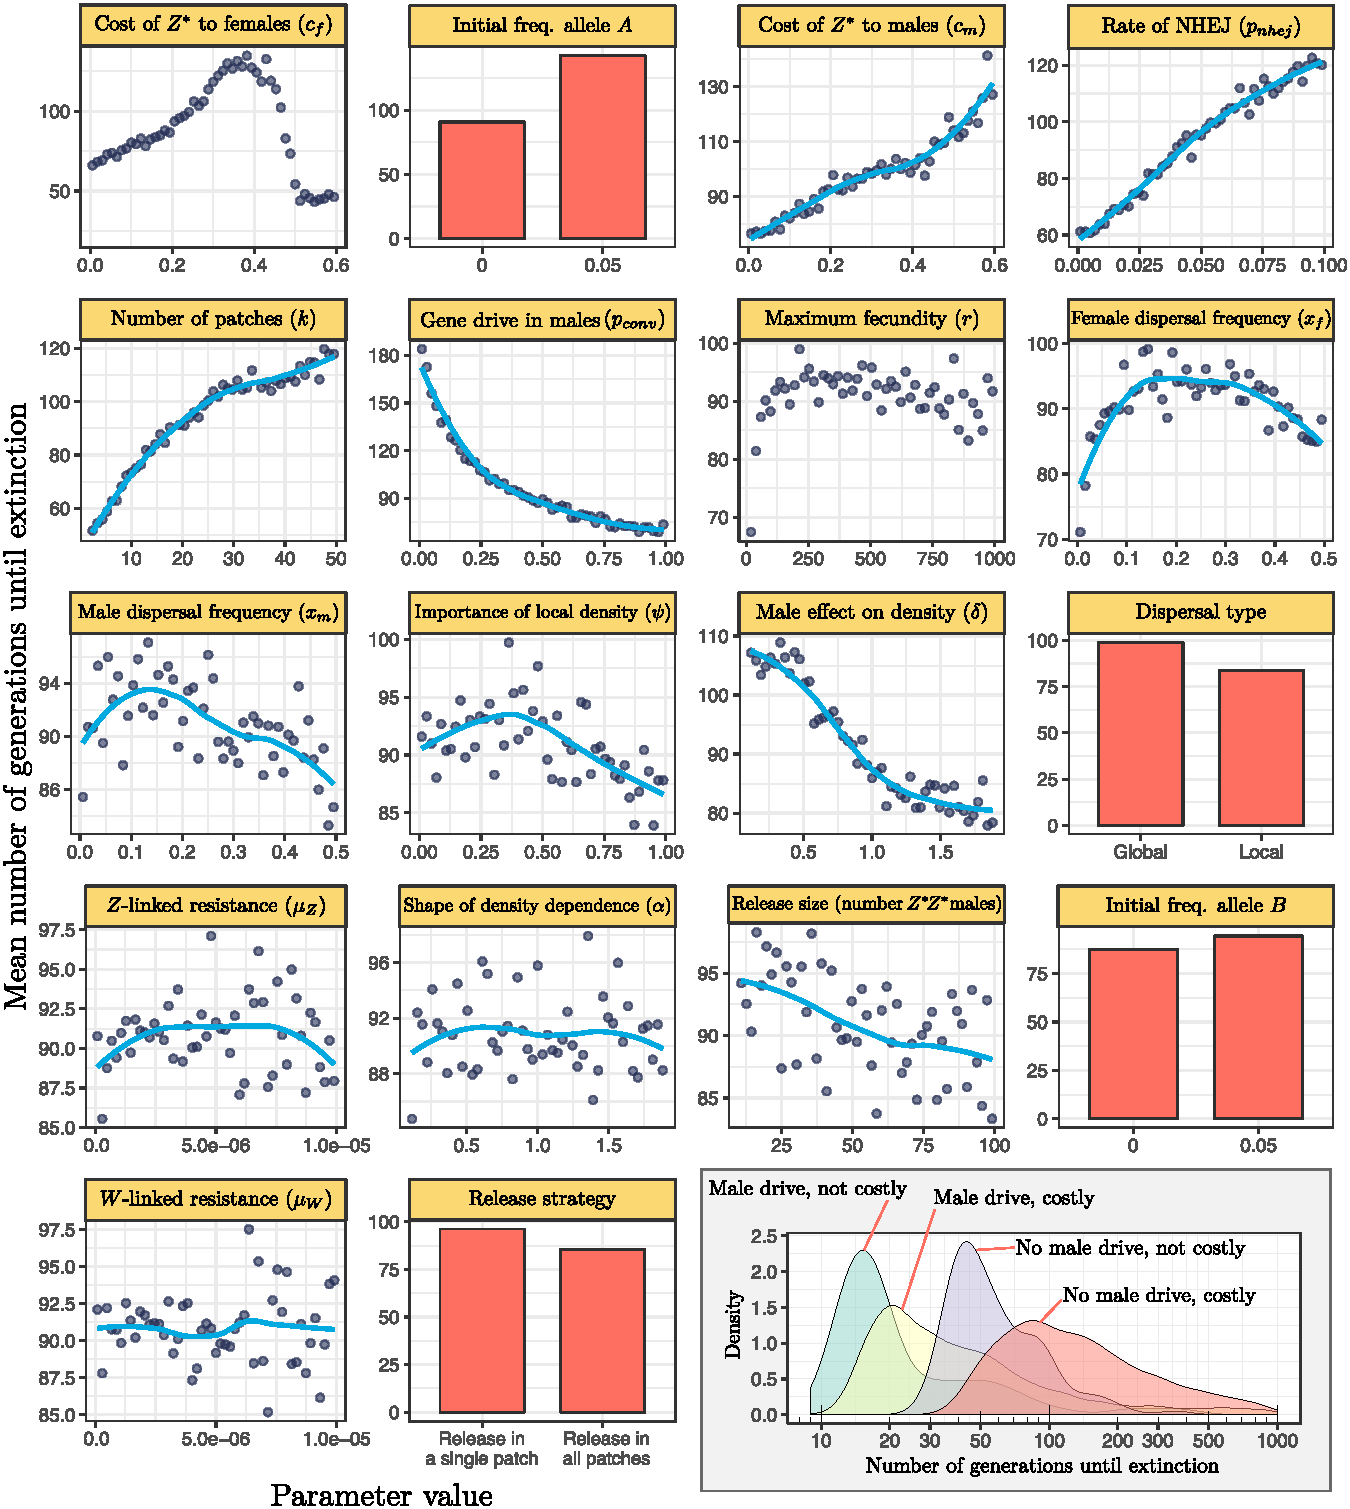
\includegraphics[width=1.0\textwidth]{../figures/fig_4_inkscape.pdf}
\caption{\footnotesize{The main plot shows the average number of generations until extinction, among the subset of runs in which extinction occurred. The density plot in the lower right shows the distribution of the response variable across all the parameter spaces in which the $Z^*$ allele was costly (defined as $c_f > 0.05$ and/or $c_m > 0.05$) or not costly ($c_f < 0.05$ and $c_m < 0.05$), and in which the $Z^*$ allele benefitted from strong gene drive in males ($p_{conv} > 0.95$) or not ($p_{conv} < 0.95$). Other details are the same as for Figure 3.}}
\end{figure}
\newpage


\dataccess{A website presenting all R scripts used to the run the simulation and
analyse the data can be found at
\url{https://lukeholman.github.io/W_shredder/}.}

\aucontribute{LH performed the analyses and wrote the manuscript.}

\competing{The author declares no conflict of interest.}

\funding{This project was stimulated by an ESEB \emph{Progress Meetings in
Evolutionary Biology} meeting, funded by grants from ESEB (European
Society for Evolutionary Biology) and from the Swiss National Science
Foundation.}


\ack{I thank the organisers (Anna Lindholm and Tom Price), funding bodies
(European Society for Evolutionary Biology; Swiss National Science
Foundation), and attendees of the 2018 ESEB \emph{Progress Meetings in
Evolutionary Biology}, which provided the impetus for this paper. I also
thank Kevin Esvelt and colleagues for describing their ongoing research
on a personal webpage; their ideas were instrumental to this paper.}

\bibliographystyle{RS}
\bibliography{references.bib}


\end{document}
